\documentclass{standalone}
\usepackage{tikz}
\usetikzlibrary{arrows.meta, positioning, shapes.geometric}

\begin{document}
	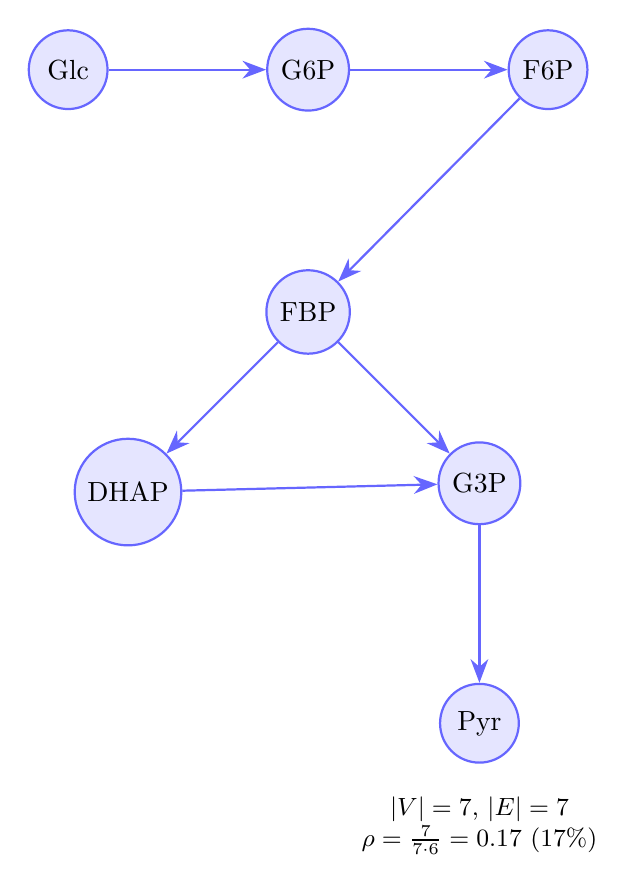
\begin{tikzpicture}[
		node distance=2cm,
		metabolite/.style={circle, draw=blue!60, fill=blue!10, thick, minimum size=1cm},
		reaction/.style={-{Stealth[length=3mm]}, thick, draw=blue!60}
		]
		% Knoten
		\node[metabolite] (glc) {Glc};
		\node[metabolite, right=of glc] (g6p) {G6P};
		\node[metabolite, right=of g6p] (f6p) {F6P};
		\node[metabolite, below=of g6p] (fbp) {FBP};
		\node[metabolite, below left=of fbp] (dhap) {DHAP};
		\node[metabolite, below right=of fbp] (g3p) {G3P};
		\node[metabolite, below=of g3p] (pyr) {Pyr};
		
		% Kanten (lineare Pfade, wenige Verbindungen)
		\draw[reaction] (glc) -- (g6p);
		\draw[reaction] (g6p) -- (f6p);
		\draw[reaction] (f6p) -- (fbp);
		\draw[reaction] (fbp) -- (dhap);
		\draw[reaction] (fbp) -- (g3p);
		\draw[reaction] (dhap) -- (g3p);
		\draw[reaction] (g3p) -- (pyr);
		
		% Dichte-Berechnung
		\node[below=0.3cm of pyr, align=center, font=\small] {
			$|V| = 7$, $|E| = 7$ \\
			$\rho = \frac{7}{7 \cdot 6} = 0.17$ (17\%)
		};
	\end{tikzpicture}
\end{document}